\documentclass[10pt]{beamer}
\usepackage{lmodern}
\usepackage[utf8]{inputenc}
\usepackage[spanish]{babel}
\usepackage{xcolor}
\usepackage{amsmath}
\usepackage{amsfonts}
\usepackage{amssymb}
\usepackage{graphicx}
\usepackage{lipsum}
\usepackage{ragged2e}
\usepackage{hyperref}
\usepackage{float}
\usepackage{url}
\usepackage{subcaption}
\usepackage{tikz}
\usetikzlibrary{positioning, arrows.meta}
\usepackage{amssymb, amsmath} % Para las fuentes de las ecuaciones


% =======================================================================
% Paquetes adicionales para mapas conceptuales integrados

\usepackage{tikz}
\usetikzlibrary{shapes.geometric, arrows.meta, positioning, fit, backgrounds}

\usetheme{Madrid}
% =======================================================================



% =======================================================================
% --- Configuración de Estilos de TikZ para los Mapas ---

\tikzset{
    box_principal/.style={rectangle, rounded corners, draw=blue!80!black, fill=blue!10, very thick, text width=3.8cm, align=center, minimum height=1cm, font=\small\bfseries},
    box_concepto/.style={rectangle, rounded corners, draw=green!60!black, fill=green!5, thick, text width=3.4cm, align=center, font=\scriptsize},
    box_ecuacion/.style={rectangle, draw=orange!80!black, fill=orange!10, thick, text width=4cm, align=center, font=\scriptsize\itshape},
    box_alerta/.style={rectangle, rounded corners, draw=red!80!black, fill=red!5, thick, text width=3.4cm, align=center, font=\scriptsize},
    box_detalle/.style={rectangle, rounded corners, draw=gray!50, fill=white, text width=3.5cm, align=center, font=\tiny},
    flecha/.style={draw, -Latex, thick, color=gray!80!black}
}
% =======================================================================


% =======================================================================
% --- Información del Autor y Título ---
\author[Andrés Rincón - Andrés Salas ]{Andrés A. Rincón Guerrero - Andrés F. Salas Ávila}
\title[Análisis de datos de flujo en redes]{Análisis de datos de flujo en redes}
\date{Junio de 2026} 
\subtitle{Análisis de redes}
%\logo{\includegraphics[scale=0.07]{imagenes/logo1.png}} % Descomentar si tienes el archivo
\institute[Universidad Nacional]{
	Universidad Nacional de Colombia \\Facultad de Ciencias\\Departamento de Estadística\\Maestría en Estadística\\
}
% =======================================================================



% =======================================================================
% --- Configuración de Secciones ---
\AtBeginSection[]
{
	\begin{frame}<beamer>{Contenido}
		\tableofcontents[currentsection,currentsubsection]
	\end{frame}
}
% =======================================================================



% =======================================================================
\begin{document}


    % Diapositiva No. 1
    % ===================================================================
	\begin{frame}
		\maketitle
	\end{frame}
    % ===================================================================



    % Diapositiva No. 2
    % ===================================================================
	\begin{frame}{Contenido}
		\tableofcontents
	\end{frame}
    % ===================================================================

    

    % Diapositiva No. 3
    % ===================================================================
    % --- SECCIÓN 1: INTRODUCCIÓN ---
    \section{Introducción al flujo en redes}
    % ===================================================================




    % Diapositiva No. 4
    % ===================================================================
    \begin{frame}{Introducción a la problemática}
        \centering
        \resizebox{\textwidth}{!}{%
        \begin{tikzpicture}[
            node distance=0.6cm and 0.8cm, 
            font=\small,
            % Estilo base
            base/.style={
                rectangle, draw, align=center, rounded corners=6pt, inner sep=8pt, thick
            },
            % Caja raíz (Título)
            box_principal/.style={
                base, fill=blue!10, font=\large\bfseries, text width=5cm
            },
            % Caja matriz (Subtítulo)
            box_matriz/.style={
                base, fill=gray!10, text width=8cm
            },
            % Cajas de los Casos (Mismo ancho y alto)
            box_concepto/.style={
                base, fill=green!5, text width=7cm, minimum height=2.5cm
            },
            box_alerta/.style={
                base, fill=green!5, text width=6.5cm, minimum height=2.5cm
            },
            % Cajas de Métodos finales (Mismo ancho y alto)
            box_metodo/.style={
                base, fill=orange!5, text width=6.5cm, minimum height=3cm, font=\footnotesize
            },
            flecha/.style={->, >=Stealth, thick, gray!80}
        ]
            
            % 1. Nodos Superiores (Centro)
            \node[box_principal] (root) {Análisis de flujos};
            
            \node[box_matriz, below=of root, yshift=0.3cm] (od) {
                \textbf{Matriz OD ($Z$)} \\[0.2cm]
                Volumen total del tráfico del origen $i$ al destino $j$.
            };
            
            % Creamos una coordenada invisible para hacer una bifurcación limpia en "Z"
            \coordinate (bifurcacion) at ([yshift=-0.5cm]od.south);
            
            % 2. Fila del Medio (Los dos casos bifurcados)
            % Los ubicamos a la izquierda y derecha de la coordenada invisible
            \node[box_concepto, left=of bifurcacion, xshift=-0.5cm, yshift=-2cm] (obs) {
                \textbf{Caso 1: Observada} \\[0.2cm]
                Toda la matriz $Z$ es medible directamente.\\
                \textit{Enfoque:} Modelar el impacto de factores externos.
            };
            
            \node[box_alerta, right=of bifurcacion, xshift=0.5cm, yshift=-2cm] (no_obs) {
                \textbf{Caso 2: No observada} \\[0.2cm]
                Es difícil o imposible medir las celdas $Z_{ij}$.\\
                \textit{Enfoque:} Estimar $Z$ usando marginales y rutas.
            };
            
            % 3. Fila Inferior (Los métodos alineados debajo de cada caso)
            \node[box_metodo, below=of obs] (grav) {
                \textbf{Modelos de gravedad} \\[0.2cm]
                Técnica inspirada en la física para predecir el flujo de interacción (como datos, llamadas o transporte) entre dos puntos en una red.
            };
            
            \node[box_metodo, below=of no_obs] (est) {
                \textbf{Estimación de matrices} \\[0.2cm]
                Técnica para estimar de dónde viene y a dónde va el tráfico total de una red cuando es imposible rastrear la ruta completa.
            };
    
            % --- CONEXIONES ---
    
            % Bajada recta desde la raíz a la matriz
            \draw[flecha] (root) -- (od);
            
            % Bifurcación desde la Matriz hacia los dos casos usando la coordenada
            \draw[flecha] (od.south) -- (bifurcacion) -| (obs.north);
            \draw[flecha] (od.south) -- (bifurcacion) -| (no_obs.north);
            
            % Bajadas rectas desde cada caso a su método
            \draw[flecha] (obs) -- (grav);
            \draw[flecha] (no_obs) -- (est);
            
        \end{tikzpicture}%
        }
    \end{frame}
    % ===================================================================



    
    % Diapositiva No. 5
    % ===================================================================
    \begin{frame}{Redes como conductos de tráfico}
        \begin{columns}[T] % Alineación superior para equilibrar el contenido
            
            % --- COLUMNA IZQUIERDA: CONTEXTO Y EJEMPLOS ---
            \begin{column}{0.4\textwidth}
                \justifying
                Muchos sistemas sirven literal o figurativamente como conductos para el movimiento de materiales, personas o información.
                
                \vspace{0.3cm}
                
                \begin{itemize}
                    \item \textbf{Redes de Transporte:} Autopistas, aerolíneas y ferrocarriles (flujo de bienes y personas).
                    \item \textbf{Redes de Comunicación:} Internet y telecomunicaciones (flujo de paquetes de datos).
                    \item \textbf{Redes Económicas:} Relaciones comerciales globales (flujo de capital).
                \end{itemize}
            \end{column}
            
            % --- COLUMNA DERECHA: IMAGEN PANORÁMICA Y DEFINICIÓN ---
            \begin{column}{0.55\textwidth}
                \centering
                % Al ser más ancha que alta, se ajusta perfectamente al ancho de esta columna
                \includegraphics[width=\textwidth]{image_001.png}
                
                \vspace{0.2cm}
            
                % Caption de la imagen
                \begin{minipage}{0.95\textwidth}
                    \scriptsize
                    \textbf{Figura No. 1:} Representación esquemática de las redes de tráfico - Imagen generada con la IA Gemini de Google (2026).
                \end{minipage}
                    
                    \vspace{0.15cm}

                
                \begin{block}{Definición}
                    \small
                    Se hará referencia al elemento constituyente de cualquier flujo de manera amplia y genérica como \textbf{tráfico}.
                \end{block}
            \end{column}
            
        \end{columns}
    \end{frame}
    % ===================================================================


    % Diapositiva No. 6
    % ===================================================================

    \begin{frame}{Formalización matemática e identificación}
        \begin{columns}[T] % Alineación superior
            
            % --- COLUMNA IZQUIERDA: CONTEXTO Y FORMALIZACIÓN ---
            \begin{column}{0.4\textwidth}
                \justifying
                Dado que los flujos poseen intrínsecamente una dirección clara, modelamos la red utilizando la teoría de grafos dirigidos:
                
                \vspace{0.3cm}
                
                \begin{itemize}
                    \item Sea $G=(V,E)$ un \textbf{digrafo}, donde los vértices $V$ representan los nodos y las aristas dirigidas $E$ se denominan \textbf{enlaces}.
                    \item El tráfico usualmente debe transitar secuencialmente a través de múltiples enlaces intermedios para trasladarse desde su origen hasta su destino final.
                \end{itemize}
            \end{column}
            
            % --- COLUMNA DERECHA: IMAGEN Y BLOQUE DE LA MATRIZ ---
            \begin{column}{0.55\textwidth}
                \centering
                % Asegúrate de cambiar 'imagen_digrafo.jpg' por el archivo real
                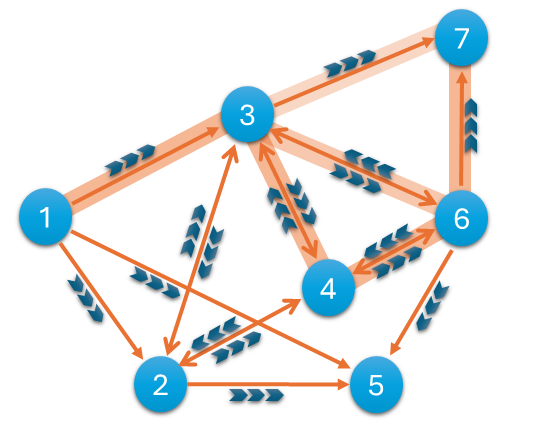
\includegraphics[width=\textwidth]{image_006.png}

                \vspace{0.2cm}

                % Caption de la imagen
                \begin{minipage}{0.95\textwidth}
                    \scriptsize
                    \textbf{Figura No. 2:} Representación esquemática de una red de flujo - Elaboración propia.
                \end{minipage}
                
                
            \end{column}
            
        \end{columns}
    \end{frame}

    % ===================================================================




    % Diapositiva No. 7
    % ===================================================================

    \begin{frame}{Formalización matemática e identificación}
        
        \centering
        
            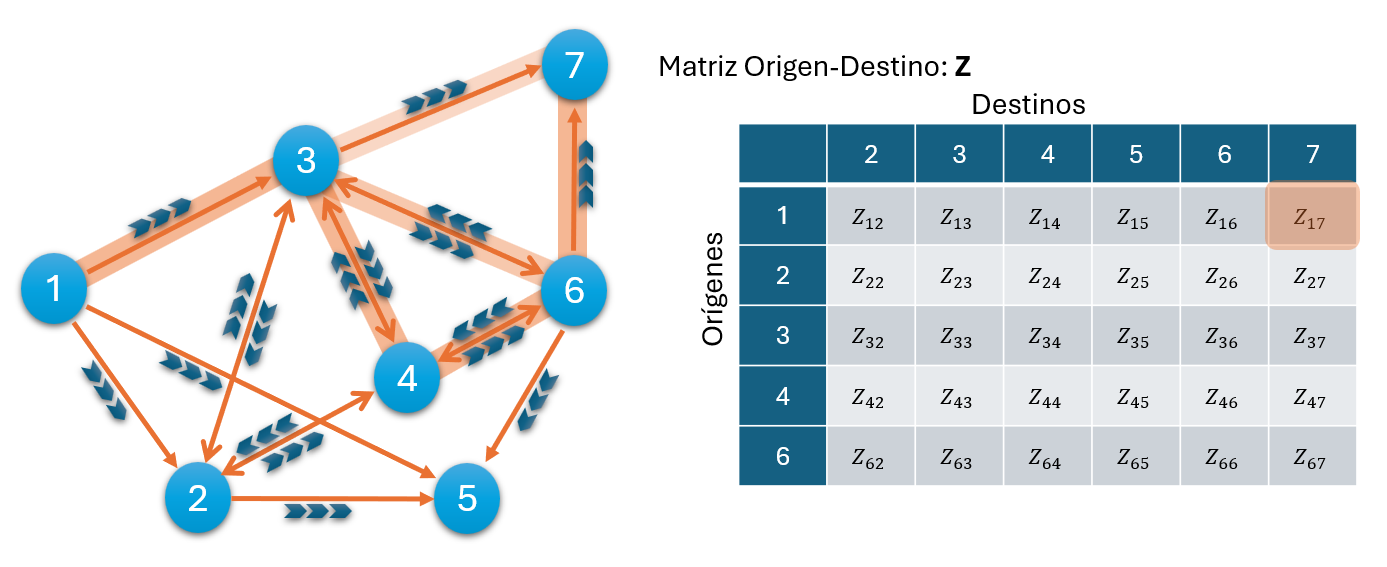
\includegraphics[width=\textwidth]{image_002.png}


            % Caption de la imagen
            \begin{minipage}{1\textwidth}
                \scriptsize
                \textbf{Figura No. 3:} Representación esquemática de una red de flujo (izquierda). Y, su matriz Origen - Destino (OD) (Derecha) - Elaboración propia.
            \end{minipage}
            
            % \vspace{0.01cm}
            
            \begin{exampleblock}{Matriz de tráfico (OD)}
                \small
                Denotada como $Z = [Z_{ij}]$, representa el volumen total de tráfico que fluye desde un vértice origen $i \in V$ hacia un destino $j \in V$ en un intervalo de tiempo específico. Es la variable fundamental de estudio.
            \end{exampleblock}
                
            
        \end{frame}
    % ===================================================================



    % ===================================================================
    % ===================================================================


    % Diapositiva No. 8
    % ===================================================================
    % --- SECCIÓN 2: MODELOS DE GRAVEDAD ---
    \section{Modelado de flujos: Modelos de gravedad}
    % ===================================================================




    % Diapositiva No. 10
    % ===================================================================

    \begin{frame}{Especificación del modelo de gravedad}
        \justifying
        
        Inspirados en la ley de gravitación universal de Newton, asumen que la intensidad de interacción entre dos poblaciones varía en proporción directa a sus tamaños e inversamente proporcional a su separación.
        
        \begin{itemize}
            \item Las variables de flujo $Z_{ij}$ se asumen como conteos independientes.
            \item Siguen distribuciones marginales de \textbf{Poisson}.
        \end{itemize}

        \begin{block}{Ecuación estructural}
            La función de media del modelo matemático se define formalmente como:
            \begin{equation}
                \mathbb{E}(Z_{ij}) = h_O(i) h_D(j) h_S(c_{ij})
            \end{equation}
            Donde $h_O$, $h_D$, y $h_S$ son funciones estrictamente positivas que representan los efectos del origen, destino y atributos de separación, respectivamente.
        \end{block}
    \end{frame}
    % ===================================================================


    
    % ===================================================================
    \begin{frame}{Linealidad y modelos lineales generalizados (GLM)}
        \justifying
        La especificación multiplicativa original del modelo presenta una enorme ventaja cuando se transforma matemáticamente a una escala logarítmica:
        
        \begin{equation}
            \log \mathbb{E}(Z_{ij}) = \log h_O(i) + \log h_D(j) + \log h_S(c_{ij})
        \end{equation}

        \begin{itemize}
            \item \textbf{Propiedad Clave:} Se transforma en una expresión lineal respecto a los parámetros desconocidos del sistema.
            \item \textbf{Inferencia:} Facilita el uso directo de la infraestructura de los Modelos Lineales Generalizados (\textbf{GLM}) bajo la familia Poisson y enlaces logarítmicos.
        \end{itemize}

        \begin{alertblock}{Aplicación Práctica: Datos de Llamadas en Austria}
            En el texto se ilustra con el dataset \texttt{calldata} ($32 \times 31 = 992$ flujos), utilizando el Producto Regional Bruto (GRP) como proxy de tamaño y distancias viales/euclidianas como costo de separación.
        \end{alertblock}
    \end{frame}
    % ===================================================================


    % Diapositiva No. 9
    % ===================================================================
    \begin{frame}{Modelo de transporte de 4 etapas}
        \centering
        
            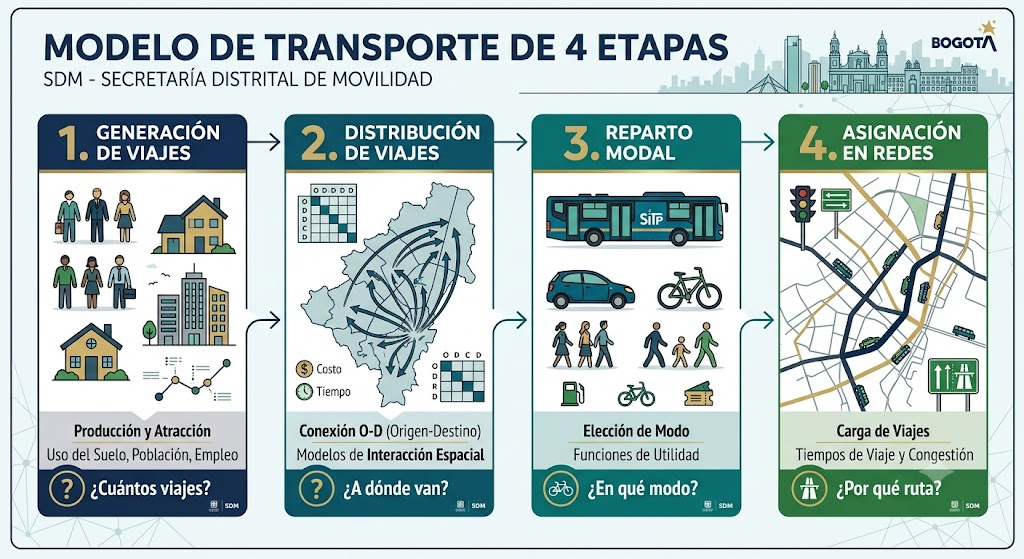
\includegraphics[width=\textwidth]{image_008.jpeg}

            \vspace{0.1cm}

            % Caption de la imagen
            \begin{minipage}{0.95\textwidth}
                \scriptsize
                \textbf{Figura No. 3:} Modelos de transporte de 4 etapas de Bogotá. - Imagen generada con la IA Gemini de Google (2026) con insumos propios.
            \end{minipage} 
    
    \end{frame}
    % ===================================================================




    % ===================================================================
    \begin{frame}{Estructura del modelo de gravedad}
        \centering
        % \resizebox ajusta automáticamente el diagrama al ancho de la diapositiva
        \resizebox{\textwidth}{!}{%
        \begin{tikzpicture}[
            node distance=0.6cm and 0.4cm, 
            font=\small,
            % Estilo base para todos los nodos
            base/.style={
                rectangle, draw, align=center, rounded corners=6pt, inner sep=7pt, thick
            },
            % Caja superior
            box_principal/.style={
                base, fill=blue!10, font=\large\bfseries, text width=4cm
            },
            % Cajas del medio (USAMOS minimum height, NO height)
            box_medio/.style={
                base, fill=green!5, text width=6cm, minimum height=2.5cm
            },
            % Cajas de abajo 
            box_detalle/.style={
                base, fill=gray!5, text width=4.5cm, minimum height=2.5cm, font=\footnotesize
            },
            flecha/.style={->, >=Stealth, thick, gray!80}
        ]

            

            
            % 1. Nodo Superior
            \node[box_principal, xshift=-3.1cm] (c2) {Modelos de gravedad};
            
            % 2. Fila del Medio 
            % Centramos la fila desplazando la primera caja un poco a la izquierda
            \node[box_medio, below=of c2, xshift=-3.1cm, yshift=-0.2cm] (eq) {
                {\large $\mathbb{E}(Z_{ij}) = h_O(i) h_D(j) h_S(c_{ij})$} \\[0.3cm] 
                Distribución: Conteo Poisson Independiente
            };
            
            \node[box_medio, right=of eq] (loglin) {
                \textbf{Linealización Logarítmica} \\[0.2cm]
                $\log \mathbb{E}(Z_{ij}) = \log h_O + \log h_D + \log h_S$ \\[0.2cm]
                Estimable mediante regresiones log-lineales.
            };
    
            % 3. Fila Inferior
            % La caja 'hd' la ponemos debajo de 'eq', pero la desplazamos a la derecha 
            % para que quede exactamente en el centro de toda la diapositiva.
            \node[box_detalle, below=of eq, xshift=2.95cm, yshift=-0.3cm] (hd) {
                \textbf{$h_D(j)$: Función de Destino} \\[0.2cm]
                Mide la capacidad de atracción.\\ Ejemplo: Demanda o población.
            };
            
            \node[box_detalle, left=of hd] (ho) {
                \textbf{$h_O(i)$: Función de Origen} \\[0.2cm]
                Mide la capacidad de emisión.\\ Ejemplo: GRP u origen económico.
            };
            
            \node[box_detalle, right=of hd] (hs) {
                \textbf{$h_S(c_{ij})$: Disuasión} \\[0.2cm]
                Mide costo de separación.\\ Decreciente con la distancia.
            };
    
            % --- CONEXIONES ---
    
            % Flecha directa al bloque de ecuación
            \draw[flecha] (c2.west) -| (eq.north);
            \draw[flecha] (eq.east) -- (loglin.west);
            
            % Conexiones en Z desde Ecuación a los tres de abajo
            % Creamos una coordenada invisible justo debajo de la ecuación para la bifurcación
            \coordinate (bajo_eq) at ([yshift=-0.4cm]eq.south);
            \coordinate (bajo_loglin) at ([yshift=-0.4cm]loglin.south);
    
            % De Ecuación a los tres de abajo con ángulos rectos (-|)
            \draw[flecha] (eq.south) -- (bajo_eq) -| (ho.north);
            \draw[flecha] (eq.south) -- (bajo_eq) -| (hd.north);
            \draw[flecha] (eq.south) -- (bajo_eq) -| (hs.north);

            % De Ecuación a los tres de abajo con ángulos rectos (-|)
            \draw[flecha] (loglin.south) -- (bajo_loglin) -| (ho.north);
            \draw[flecha] (loglin.south) -- (bajo_loglin) -| (hd.north);
            \draw[flecha] (loglin.south) -- (bajo_loglin) -| (hs.north);
    
        \end{tikzpicture}%
        } % Cierre del \resizebox
    \end{frame}
    % ===================================================================
    % ===================================================================


    % ===================================================================
    % ===================================================================
    % --- SECCIÓN 3: INFERENCIA PARA MODELOS DE GRAVEDAD ---
    \section{Inferencia para modelos de gravedad}

    \begin{frame}{Estimación por Máxima Verosimilitud y GLM}
        \justifying
        Dado que se asume que los flujos $Z_{ij}$ son variables independientes con distribución de Poisson, el marco natural para estimar los parámetros es la \textbf{Máxima Verosimilitud}.
        
        \begin{itemize}
            \item \textbf{Implementación Computacional:} Gracias a la linealización logarítmica, el modelo de gravedad es un caso específico de la familia de Modelos Lineales Generalizados (GLM).
            \item \textbf{Ecuación Log-Lineal Típica:}
            \begin{equation}
                \log \mu_{ij} = \alpha_i + \beta_j + \theta^T c_{ij}
            \end{equation}
            \item El ajuste utiliza algoritmos iterativos de mínimos cuadrados reponderados (Newton-Raphson), comunes en software como R (\texttt{glm}).
        \end{itemize}
    \end{frame}
    % ===================================================================


    
    % ===================================================================
    \begin{frame}{Evaluación del Ajuste del Modelo}
        \justifying
        Para evaluar qué tan bien captura el modelo la realidad de los flujos, se utilizan dos herramientas clave:
        
        \begin{block}{Criterio de Información de Akaike (AIC)}
            Sirve para comparar modelos competidores. Penaliza la complejidad (número de variables) para evitar el sobreajuste (\textit{overfitting}). Un AIC menor indica un mejor modelo.
        \end{block}

        \begin{block}{Análisis de Error Relativo}
            Permite medir la precisión comparando el valor estimado frente al valor observado:
            \begin{equation}
                \text{Error Relativo} = \frac{Z_{ij} - \hat{\mu}_{ij}}{Z_{ij}}
            \end{equation}
            En la práctica, los modelos de gravedad suelen subestimar flujos muy altos y sobreestimar flujos muy bajos.
        \end{block}
    \end{frame}
    % ===================================================================



    % ===================================================================
    \section{Estimación de matrices: Un problema inverso}

    \begin{frame}{El Desafío de la Estimación de Tráfico}
        \justifying
        En escenarios reales (como redes de carreteras nacionales o enrutadores principales de Internet), medir directamente el flujo origen-destino $Z_{ij}$ es prohibitivo o técnicamente imposible.
        
        \begin{itemize}
            \item \textbf{Lo Observable:} Contar vehículos o paquetes que transitan físicamente por los enlaces locales ($X_e$) es sumamente sencillo mediante sensores o contadores.
            \item \textbf{El Objetivo:} Deducir o realizar la ingeniería inversa de los flujos agregados $Z$ a partir únicamente de las mediciones de los enlaces $X$.
        \end{itemize}

        \begin{exampleblock}{La ecuación de enrutamiento fundamental}
            \begin{equation}
                X = B Z
            \end{equation}
            Donde $X$ es el vector de flujos en enlaces, $Z$ es la matriz de tráfico expresada en forma de vector, y $B$ es la \textbf{matriz de enrutamiento} (indica si un par $ij$ atraviesa el enlace $e$).
        \end{exampleblock}
    \end{frame}
    % ===================================================================



    % ===================================================================
    \begin{frame}{¿Por qué es un problema mal planteado?}
        \justifying
        El núcleo matemático del problema radica en las dimensiones del sistema algebraico planteado por la relación $X = BZ$:
        
        \begin{itemize}
            \item El número de enlaces observables ($N_e$, filas de $B$) es sustancialmente **menor** que el número de pares origen-destino posibles ($I \times J$, columnas de $B$).
            \item El sistema de ecuaciones resultante es algebraicamente \textbf{subdeterminado}.
        \end{itemize}

        \begin{alertblock}{Consecuencia matemática}
            No existe una solución única. El problema es \textbf{altamente indeterminado} e incomprensible sin añadir restricciones extras: existe un número infinito de matrices $Z$ distintas que pueden reproducir exactamente el mismo vector de enlaces $X$.
        \end{alertblock}
        \small Para resolver esta ambigüedad teórica, los métodos estáticos modernos recurren a penalizaciones o regularizaciones de entropía combinadas con modelos de gravedad (como el método de \textit{Tomogravity}).
    \end{frame}
    % ===================================================================


    % ===================================================================
    \begin{frame}{Mapa Conceptual: El Problema Inverso de Estimación}
        \centering
        \resizebox{\textwidth}{!}{%
        \begin{tikzpicture}[
            node distance=0.6cm and 0.4cm, 
            font=\small,
            % Estilos base
            base/.style={
                rectangle, draw, align=center, rounded corners=6pt, inner sep=8pt, thick
            },
            box_principal/.style={
                base, fill=purple!10, draw=purple!80!black, font=\large\bfseries, text width=5.5cm
            },
            box_ecuacion/.style={
                base, fill=blue!5, text width=4cm, minimum height=1cm
            },
            % Cajas de las variables (Mismo alto para simetría: 2.8cm)
            box_concepto/.style={
                base, fill=gray!5, text width=3.4cm, minimum height=2cm, font=\footnotesize
            },
            box_alerta/.style={
                base, fill=red!10, draw=red!80!black, text width=3.4cm, minimum height=2cm, font=\footnotesize
            },
            % Caja inferior ancha
            box_final/.style={
                base, fill=red!5, draw=red!80!black, text width=8.5cm, font=\footnotesize
            },
            flecha/.style={->, >=Stealth, thick, gray!80}
        ]
            
            % 1. Nodo Ecuación (Ancla central)
            \node[box_ecuacion] (eq2) {
                {\Large $X = B \times Z$}
            };
            
            % 2. Nodo Superior (Alineado exactamente arriba de la ecuación)
            \node[box_principal, above=of eq2, yshift=0.1cm] (c3) {Estimación de matrices};
            
            % 3. Fila del Medio (Las 3 variables de la ecuación)
            \node[box_concepto, below=of eq2, yshift=-0.3cm] (b_node) {
                \textbf{Matriz $B$ (Conocida)} \\[0.2cm]
                Estructura de enrutamiento y topología de caminos.
            };
            
            \node[box_concepto, left=of b_node] (x_node) {
                \textbf{Vector $X$ (Conocido)} \\[0.2cm]
                Flujos observados sobre los enlaces físicos de la red.
            };
            
            \node[box_alerta, right=of b_node] (z_node) {
                \textbf{Vector $Z$ (Incógnita)} \\[0.2cm]
                Flujos OD desagregados que se desean predecir.
            };
            
            % 4. Nodo Final (Problema indeterminado)
            \node[box_final, below=of b_node, yshift=-0.1cm] (ill) {
                \textbf{Naturaleza inversa e indeterminada} \\[0.2cm]
                Dado que $\text{Filas de } B \ (N_e) \ll \text{Columnas de } B \ (I \times J)$, el problema está subdeterminado. Existen \textbf{infinitas soluciones} posibles para $Z$.
            };
    
            % --- CONEXIONES ---
    
            % Flecha principal baja recta
            \draw[flecha] (c3) -- (eq2);
            
            % Conexiones en Z hacia las 3 variables
            \coordinate (bajo_eq) at ([yshift=-0.4cm]eq2.south);
            \draw[flecha] (eq2.south) -- (bajo_eq) -| (x_node.north);
            \draw[flecha] (eq2.south) -- (bajo_eq) -| (b_node.north); % Aunque esta es central, -| la mantiene recta
            \draw[flecha] (eq2.south) -- (bajo_eq) -| (z_node.north);
            
            % Flecha final hacia la conclusión
            \draw[flecha] (b_node.south) -- (ill.north);
            
        \end{tikzpicture}%
        }
    \end{frame}
    % ===================================================================
    % ===================================================================



    % ===================================================================
    % ===================================================================
    % --- SECCIÓN 4: EL MÉTODO TOMOGRAVITY ---
    \section{El Método Tomogravity (Sec. 9.3.2)}

    \begin{frame}{Regularización del Problema Inverso}
        \justifying
        Para solucionar el problema subdeterminado ($X = BZ$), el método \textbf{Tomogravity} incorpora una penalización al modelo de mínimos cuadrados. 
        
        \begin{alertblock}{Minimización de Mínimos Cuadrados Penalizados}
            Se busca el vector de flujos $\mu$ que minimice la siguiente función objetivo:
            \begin{equation}
                ||x - B\mu||^2 + \lambda D(\mu || \mu^{(0)})
            \end{equation}
        \end{alertblock}

        \begin{itemize}
            \item $||x - B\mu||^2$: Ajuste a los datos observados en los enlaces.
            \item $D(\mu || \mu^{(0)})$: Divergencia de \textbf{Kullback-Liebler} (entropía relativa). Penaliza soluciones que se alejen demasiado de un modelo a priori $\mu^{(0)}$.
            \item $\lambda$: Parámetro de suavizado que controla el peso de la penalización.
        \end{itemize}
    \end{frame}
    % ===================================================================



    % ===================================================================
    \begin{frame}{Construcción del A Priori y Ajuste Final}
        \justifying
        El término "Tomogravity" nace de combinar la Tomografía de Redes con un Modelo de Gravedad inicial.
        
        \begin{itemize}
            \item \textbf{El Modelo Base ($\mu^{(0)}$):} Se define asumiendo que el tráfico es simplemente el producto del flujo total de salida del origen y el flujo total de entrada del destino (un modelo de gravedad simple).
        \end{itemize}

        \begin{exampleblock}{Ajuste Proporcional Iterativo (IPFP)}
            Si las mediciones de los enlaces $X$ no tienen error, la estimación $\hat{\mu}$ obtenida de la regularización debe ajustarse forzosamente para cumplir la restricción dura $X = B\hat{\mu}$. 
            
            Para esto se utiliza el \textbf{IPFP} (Ajuste Proporcional Iterativo), forzando a que las celdas estimadas coincidan perfectamente con los márgenes medidos.
        \end{exampleblock}
    \end{frame}
    % ===================================================================



    % ===================================================================
    \begin{frame}{Mapa Conceptual: El Flujo de Tomogravity}
        \centering
        \begin{tikzpicture}[node distance=0.6cm and 0.4cm, scale=0.75, transform shape]
            \node[box_principal, fill=purple!10, draw=purple!80!black] (c4) {Método Tomogravity\\(Sec. 9.3.2)};
            
            \node[box_concepto, below left=of c4, xshift=-1cm] (ls) {\textbf{Datos Observados}\\Minimizar error de enlaces:\\$||x - B\mu||^2$};
            \node[box_concepto, below right=of c4, xshift=1cm] (prior) {\textbf{Conocimiento Previo}\\Modelo de Gravedad base ($\mu^{(0)}$)};
            
            \node[box_ecuacion, below=of c4, yshift=-1.5cm, text width=6cm] (obj) {\textbf{Función Objetivo Combinada}\\Minimizar: $||x - B\mu||^2 + \lambda D(\mu || \mu^{(0)})$\\ \tiny (Donde $D$ es Divergencia Kullback-Liebler)};
            
            \node[box_detalle, below=of obj] (ipfp) {\textbf{Post-Procesamiento (IPFP)}\\Ajuste Proporcional Iterativo para forzar que los flujos resultantes cumplan estrictamente $X = BZ$.};

            \draw[flecha] (c4) -- (ls.north);
            \draw[flecha] (c4) -- (prior.north);
            \draw[flecha] (ls.south) -- (obj.north west);
            \draw[flecha] (prior.south) -- (obj.north east);
            \draw[flecha] (obj.south) -- (ipfp.north);
        \end{tikzpicture}
    \end{frame}
    % ===================================================================






    
    

\end{document}